% =============================================================================
%  QUOKKAGUARD paper 003 — Tamper-Evident Action Provenance for Confidential
%  Clinical AI Agents. House style derived from papers/_template (QFIRE format).
%  Build:  make paper   (tectonic preferred).
% =============================================================================
\documentclass[11pt]{article}
\usepackage[utf8]{inputenc}
\usepackage[margin=1in]{geometry}
\usepackage{booktabs}
\usepackage{graphicx}
\usepackage{float}
\usepackage{afterpage}
\usepackage[section]{placeins}
\renewcommand{\topfraction}{0.9}
\renewcommand{\bottomfraction}{0.8}
\renewcommand{\textfraction}{0.08}
\renewcommand{\floatpagefraction}{0.75}
\setcounter{topnumber}{3}
\setcounter{bottomnumber}{2}
\setcounter{totalnumber}{5}
\usepackage{amsmath}
\usepackage{amssymb}
\usepackage{hyperref}
\usepackage{xcolor}
\usepackage{listings}
\definecolor{kwblue}{rgb}{0.10,0.20,0.65}
\definecolor{typepurple}{rgb}{0.50,0.15,0.55}
\definecolor{strred}{rgb}{0.62,0.12,0.12}
\definecolor{cmtgreen}{rgb}{0.20,0.45,0.20}
\lstdefinestyle{housespecyaml}{
  basicstyle=\ttfamily\footnotesize,
  backgroundcolor=\color{black!3},
  frame=single, framesep=5pt, rulecolor=\color{black!45},
  columns=fullflexible, breaklines=true, keepspaces=true, showstringspaces=false,
  alsoletter=_,
  commentstyle=\color{cmtgreen}\itshape,
  stringstyle=\color{strred},
  morecomment=[l]{\#}, morestring=[b]", morestring=[b]',
  keywordstyle=\color{kwblue}\bfseries,
  keywords={seq,ts,kind,body,prev_hash,this_hash,sig,merkle_root,mode},
  keywordstyle=[2]\color{typepurple}\bfseries,
  keywords=[2]{header,decision,mutation,checkpoint,chained_signed},
}
\lstdefinestyle{housespecyamlbare}{style=housespecyaml, frame=none,
  backgroundcolor=\color{white}, xleftmargin=0pt, framexleftmargin=0pt,
  aboveskip=1pt, belowskip=0pt}
\usepackage[most]{tcolorbox}
\tcbuselibrary{listings,skins}
\usepackage{tikz}
\usetikzlibrary{positioning,shapes.geometric,arrows.meta,calc,fit,backgrounds,shadows}
\definecolor{cardindigo}{HTML}{4F46E5}
\definecolor{slate}{HTML}{475569}
\definecolor{amber}{HTML}{D97706}
\definecolor{cardblue}{HTML}{1D4ED8}
\definecolor{cardpurple}{HTML}{6D28D9}
\definecolor{cardteal}{HTML}{0F766E}
\tcbset{
  cardcol/.store in=\cardcol, cardcol=cardblue,
  policycard/.style={
    enhanced, breakable=false, arc=3pt, boxrule=0.7pt, top=3pt, bottom=3pt,
    left=7pt, right=7pt, boxsep=1pt, coltitle=white,
    colframe=\cardcol!60!black, colback=white, colbacktitle=\cardcol,
    fonttitle=\bfseries\small, drop fuzzy shadow=black!25,
  },
}
\usepackage{url}
\usepackage{multirow}
\usepackage{array}
\usepackage{ragged2e}
\newcolumntype{L}[1]{>{\RaggedRight\arraybackslash}p{#1}}
\usepackage[htt]{hyphenat}
\hypersetup{colorlinks=true, linkcolor=blue, citecolor=blue, urlcolor=blue}

\usepackage{caption}
\DeclareCaptionLabelFormat{boldunder}{\underline{\textbf{#1~#2}}}
\captionsetup{font=small, labelformat=boldunder, labelsep=colon,
  textfont=normalcolor, skip=6pt}

\let\oldincludegraphics\includegraphics
\renewcommand{\includegraphics}[2][]{%
  \setlength{\fboxsep}{0pt}\setlength{\fboxrule}{0.5pt}%
  \fbox{\oldincludegraphics[#1]{#2}}}

\providecommand{\NumPrompts}{0}
\providecommand{\NumAttacks}{0}
\providecommand{\NumBenign}{0}
\IfFileExists{numbers.tex}{% Headline numbers for paper 003, from the 2026-06-08 stage-4 run
% (macOS/APFS dev laptop). Source artifacts: results/003-tamper-audit/*/summary.json
% and docs/superpowers/specs/2026-06-08-003-*-results.md. Every reported number in
% main.tex resolves to a macro here, so the prose stays traceable to the run.
%
% Core macros providecommand'd in main.tex -> override with \renewcommand.
\renewcommand{\NumPrompts}{200}      % entries in the E1 fixture log
\renewcommand{\NumAttacks}{26}       % tampered logs in the E1 corpus

% --- E1/E5 detection + localization ---
\newcommand{\TDR}{100\%}             % tamper detection rate (26/26)
\newcommand{\TDRcount}{26/26}
\newcommand{\LOCrate}{100\%}         % localization on point-tamper classes (20/20)
\newcommand{\LOCcount}{20/20}

% --- E2 write cost (median per entry) ---
\newcommand{\ComputeUs}{14.0}        % compute-only (blake3+ed25519, no fsync), microseconds
\newcommand{\ComputeThru}{71{,}400}  % entries/s/core from compute-only
\newcommand{\PlainUs}{42.6}          % plain v1 baseline, microseconds (no fsync)
\newcommand{\ChainedMs}{4.95}        % chained, milliseconds (per-entry fsync)
\newcommand{\ChainedSignedMs}{4.71}  % chained_signed, milliseconds
\newcommand{\FsyncMs}{4.7}           % per-entry fsync durability tax, milliseconds
\newcommand{\NvmeLo}{64}             % NVMe-class projection low, microseconds
\newcommand{\NvmeHi}{214}            % NVMe-class projection high, microseconds

% --- E3 anchor cadence sweep (N=20,000 entries) ---
\newcommand{\AnchorN}{20{,}000}
\newcommand{\OverheadKten}{5.84\%}   % storage overhead at k=10
\newcommand{\OverheadKhund}{0.58\%}  % at k=100
\newcommand{\OverheadKthou}{0.058\%} % at k=1000
\newcommand{\OverheadKtenk}{0.006\%} % at k=10000
\newcommand{\WindowKthou}{13}        % detection window at k=1000

% --- E4 verify scaling ---
\newcommand{\VerifyThru}{458{,}000}        % unsigned chain, entries/s, roughly flat
\newcommand{\VerifyThruSigned}{251{,}000}  % per-entry signed via parallel+batch default, entries/s
\newcommand{\VerifyOneM}{2.18}             % unsigned verify time at 1e6 entries, seconds

% --- system facts ---
\newcommand{\EntryBytes}{465}        % measured signed entry size, bytes
\newcommand{\AuditTests}{37}         % audit-module unit tests
}{}

\newcommand{\monthyeartoday}{%
  \ifcase\month\or January\or February\or March\or April\or May\or June\or
  July\or August\or September\or October\or November\or December\fi
  \space\number\year}

\begin{document}

% ============================================================================
\thispagestyle{empty}
\noindent
\begin{minipage}[c]{0.55\textwidth}
  \raggedright\oldincludegraphics[height=1.05cm]{figs/quome.png}
\end{minipage}\hfill
\begin{minipage}[c]{0.4\textwidth}
  \raggedleft\itshape\large \monthyeartoday
\end{minipage}

\vspace{1.1em}
\begin{center}
  {\LARGE\bfseries Tamper-Evident Action Provenance\\[2pt]
   for Confidential Clinical AI Agents\par}

  \vspace{0.7em}
  {\large James Schwoebel\par}

  \vspace{0.4em}
  {\small Quome Inc.\par}
  \vspace{0.35em}
\end{center}

\vspace{0.5em}
\begin{tcolorbox}[breakable, enhanced jigsaw, colback=black!4, colframe=black!4,
  arc=5pt, boxrule=0pt, left=16pt, right=16pt, top=10pt, bottom=10pt]
\setlength{\parskip}{0pt}
{\centering\large\bfseries Abstract\par}
\smallskip
\fontsize{9.5}{11.3}\selectfont
Clinical-AI governance demands a complete, attributable record of every action an
agent takes. Yet the prior systems in this program stored that record as a plain
JSONL file (QFIRE~\cite{schwoebel2026qfire}) and an in-memory hash chain
(quanchor~\cite{pristineweights2026}): an adversarial agent, a compromised host
process, or a privileged operator can silently rewrite, drop, or reorder entries,
defeating the very traceability the framework requires (HAARF~C2~\cite{schwoebel2026haarf}).
We close this third zero-trust gap --- after attested weights and an attested
harness --- with a single tamper-evident log that unifies the gateway decision
stream and the harness mutation stream into one \textbf{blake3-chained,
ed25519-signed, externally-anchored, append-only} record, plus a streaming verifier
that localizes the first tampered entry. We introduce \textbf{TamperBench}, a
labeled corpus of six audit-tampering attack classes (TA1--TA6), and show the
verifier detects \TDR{} of tampering (\TDRcount{}) and localizes point tampers at
\LOCrate{}. The cryptographic cost is small --- \ComputeUs~\textmu s/entry
($\sim$\ComputeThru~entries/s/core) --- so the observed chained write latency is
dominated by per-entry \texttt{fsync}, the correct fail-closed durability semantic;
verification is linear at $\sim$\VerifyThru~entries/s. The central result: making a
clinical agent's action record \emph{non-repudiable and tamper-evident} costs
microseconds of computation and is achievable at deployment scale. All code,
datasets, and result artifacts are released; all data are synthetic.

\medskip
\noindent\textbf{Keywords:}~tamper-evident logging; audit provenance; hash chains;
Merkle anchoring; clinical AI safety; confidential computing; non-repudiation.

\medskip
\noindent\textcolor{blue}{\textbf{Framework:}}~implements HAARF control~C2 (primary); C8.1.5, C8.4.3 secondary~\cite{schwoebel2026haarf} --- the Healthcare AI Agents Regulatory Framework, the source of the QUOKKAGUARD program.\\
\noindent\textcolor{blue}{\textbf{Code \& data:}}~\href{https://github.com/quome-cloud/quledger}{\texttt{github.com/quome-cloud/quledger}}\\
\noindent\textcolor{blue}{\textbf{Correspondence:}}~\href{mailto:jim@quome.com}{jim@quome.com}
\end{tcolorbox}

\vspace{0.3em}

% ============================================================================
\section{Introduction}
A deployed clinical AI agent is trusted to act: it orders medications, requests
labs, triages patients, and writes to the record. Every regulatory and governance
regime that contemplates such agents --- HIPAA technical safeguards, which mandate
audit controls and integrity protection for electronic health
information~\cite{hipaa164312}; the FDA's 21~CFR Part~11 expectation of timestamped,
attributable, tamper-resistant electronic records~\cite{cfr11}; ONC certification;
FDA Software-as-a-Medical-Device expectations~\cite{fdapccp}; the NIST AI Risk
Management Framework's emphasis on accountability and
traceability~\cite{nistairmf}; the EU AI Act's record-keeping obligations for
high-risk systems~\cite{euaiact}; and the HAARF framework's traceability category
(C2)~\cite{schwoebel2026haarf} --- requires a \emph{complete and attributable record of what
the agent did}. HAARF C2, in particular, demands an unbroken, machine-interpretable
\emph{decision lineage} linking every input, output, and tool execution to an
authenticated identity. That record is the substrate of every post-incident review,
every malpractice or regulatory inquiry, and every claim that an autonomous system
behaved within its sanctioned scope.

Zero-trust accountability for a clinical agent rests on three pillars:
\emph{attested weights} (confidential computing attests what a model is),
\emph{attested harness} (sandboxing and capability tokens bound what the runtime
can do), and an \emph{attested log} (a tamper-evident record of what actually
happened). This program has hardened the first two already. QFIRE~\cite{schwoebel2026qfire}
firewalls the agent$\leftrightarrow$tool path with purpose-scoped rules;
quanchor~\cite{pristineweights2026} adds attestation-rooted harness defenses,
showing that confidential computing attests \emph{what a model is} (its weights)
but not \emph{what its harness makes it do}. The third pillar is the gap: attested
weights and harnesses constrain behavior \emph{during} execution but do not
guarantee the permanence or truthfulness of the resulting historical record. Both
prior systems, in fact, recorded their own decisions in mutable storage: QFIRE in a
plain JSONL append file, quanchor's provenance ledger in an in-memory hash chain
that is never persisted. A plain file is rewritable by anyone with disk access; an
in-memory chain vanishes on restart and is invisible to an external auditor. The
audit log --- the one artifact whose integrity the whole governance story depends
on --- is the weakest link.

\begin{figure}[htb]
\centering
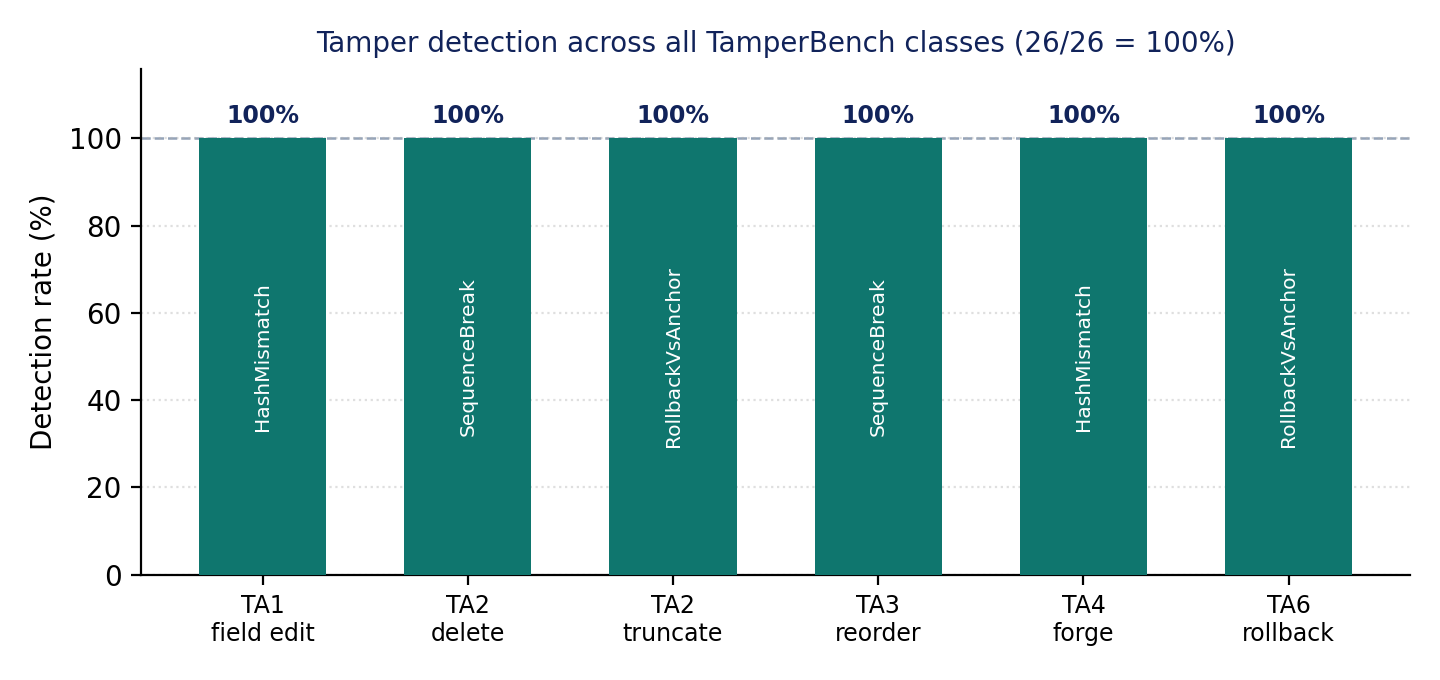
\includegraphics[width=0.95\linewidth]{figs/detection.png}
\caption{\textbf{The paper in one figure.} Across all six TamperBench attack classes
(\NumAttacks{} tampered logs), the streaming verifier detects \TDR{} of tampering.
Each bar is annotated with the verifier's diagnosis: in-place edits and forgeries
break the blake3 hash (\textsc{HashMismatch}), deletion and reordering break the
sequence (\textsc{SequenceBreak}), and truncation/rollback are caught only by the
external anchors (\textsc{RollbackVsAnchor}) --- exactly the mechanism each attack
targets.}
\label{fig:hero}
\end{figure}

We make the action record itself tamper-evident. The contribution is a single log
(\S\ref{sec:design}) that unifies the gateway decision stream and the harness
mutation stream into one append-only structure where every entry is chained to its
predecessor by a blake3 hash over the exact bytes written, signed with ed25519, and
periodically committed to an external anchor. A streaming verifier walks the log,
checks chain, signatures, and anchors, and reports the first broken entry with a
classification of the tamper. The design follows the transparency-log lineage
(timestamping~\cite{haber1991timestamp}, Merkle trees~\cite{merkle1987},
Certificate Transparency~\cite{rfc6962,trillian}) specialized to an in-enclave
gateway hot path.

\paragraph{Contributions.}
\begin{enumerate}
  \item \textbf{The central result.} Making a clinical agent's action record
  tamper-evident and non-repudiable costs $\sim$\ComputeUs~\textmu s of computation
  per entry and detects \TDR{} of tampering with exact localization
  (\S\ref{sec:results}).
  \item \textbf{The system.} A blake3-chained, ed25519-signed, externally-anchored,
  single-writer fail-closed log (\texttt{src/audit/}) that unifies decisions and
  harness mutations and ships a localizing verifier (\S\ref{sec:design}).
  \item \textbf{TamperBench.} A labeled, reusable corpus of six audit-tampering
  attack classes with ground truth, able to benchmark \emph{any} audit-integrity
  scheme, released Apache-2.0 and fully synthetic (\S\ref{sec:benchmark}).
  \item \textbf{Deployment evidence.} A measured cost model separating the small
  cryptographic overhead from the (hardware-bound) durability cost, plus a security
  argument mapping each adversary tier to a defended mechanism (\S\ref{sec:results},
  \S\ref{sec:security}).
  \item \textbf{Head-to-head and a verification speedup.} A quantitative comparison against other
  tamper-evident-log constructions and real libraries (Certificate Transparency / \texttt{ct-merkle},
  \texttt{rs\_merkle}) on identical primitives---our construction is the only one combining per-entry
  localization, public non-repudiation, and rollback (\S\ref{sec:compare})---and a parallel+batch verifier
  that makes per-entry-signed verification $\sim$23$\times$ faster (now the default) with identical
  guarantees (\S\ref{sec:fastverify}).
\end{enumerate}

\paragraph{Positioning.} Unlike transparency logs designed for a separate
log-server trust domain~\cite{rfc6962,trillian} or signed-syslog
streams~\cite{rsyslogsign}, our log runs \emph{inside} the same attested workload as
the agent and gateway, on the synchronous decision path, under a threat model in
which the host operator is untrusted. The default production deployment is a
confidential enclave (e.g.\ GCP Confidential Space~\cite{confidentialspace}); the
signing key is released to the workload via attestation, mirroring the goal-anchor
key handling of quanchor~\cite{pristineweights2026,teepartition2023}.

% ============================================================================
\section{Threat Model and Positioning}\label{sec:threat}
\paragraph{Adversary.} We consider three tiers, in increasing privilege: (i) the
\emph{agent} itself, which may be adversarial or hijacked and wishes to erase or
alter the record of an unsafe action; (ii) a \emph{co-located process} sharing the
host; and (iii) a \emph{privileged operator} with direct read/write access to the
log store. The host operating system and storage are untrusted (the confidential
enclave model): an attacker at tier (iii) can replace arbitrary bytes of the log
file or roll the entire store back to an earlier snapshot.

\paragraph{Attack classes (TamperBench).} We enumerate six concrete tampers:
\textbf{TA1} entry mutation (alter a recorded field, e.g.\ the ordered drug or
dose); \textbf{TA2} deletion or tail truncation (drop an incriminating action);
\textbf{TA3} reordering (fabricate a benign causal story); \textbf{TA4}
forgery/backdating (insert fabricated entries); \textbf{TA5} repudiation (deny
having performed a recorded action); and \textbf{TA6} host-level rollback (replace
the store with an earlier consistent snapshot).

\paragraph{What is and is not defended.} The hash chain plus per-entry signatures
make TA1--TA5 \emph{detectable} against all three tiers \emph{up to a full-file
rewrite}: an attacker who controls the entire file and the signing key could
re-emit a self-consistent log. Two mechanisms close that gap. External anchoring
defeats TA6 (and tail truncation) because the attacker cannot also roll back an
append-only sink on a separate trust domain. Out-of-band key knowledge (a verifier
invoked with a pinned public key, \texttt{-{}-pubkey}) defeats the re-key /
mode-downgrade variant, because a log re-signed under the attacker's key fails
verification against the real key. This boundary is stated explicitly in the
verifier's contract and revisited in \S\ref{sec:security} and
\S\ref{sec:limitations}.

\begin{table}[htb]\centering\small
\begin{tabular}{L{3.0cm}L{4.3cm}L{4.3cm}}
\toprule
System & Approach & Gap this paper targets \\
\midrule
QFIRE~\cite{schwoebel2026qfire} & plain JSONL append log of decisions & mutable by anyone with disk access \\
quanchor~\cite{pristineweights2026} & in-memory SHA-256 provenance chain of MIIM mutations & not persisted; no signatures; no external auditor \\
Certificate Transparency / Trillian~\cite{rfc6962,trillian} & Merkle transparency log in a separate server domain & not on an in-enclave synchronous decision path; separate trust domain assumed \\
Signed syslog~\cite{rsyslogsign} & per-message MAC/signature stream & no chain localization, no rollback anchoring, no unified decision+mutation record \\
\textbf{This work} & unified blake3-chain + ed25519 + anchored log, in-enclave, localizing verifier & --- \\
\bottomrule
\end{tabular}
\caption{Positioning against representative recent systems and the two prior papers
in this program.}
\label{tab:related}
\end{table}

% ============================================================================
\section{System Design}\label{sec:design}
\subsection{Overview}
The log is a sequence of JSONL lines, one per event, written by a single writer
that owns the chain head. Four entry \emph{kinds} share one format: a
\texttt{header} (sequence 0: format version, signing public key, mode); a
\texttt{decision} (a gateway Allow/Block/Transform/Escalate, the QFIRE record); a
\texttt{mutation} (a harness/MIIM change, the QUOKKAGUARD provenance record); and a
\texttt{checkpoint} (a batched Merkle-root signature). Unifying both streams into
one chain preserves the causal order between a decision and the mutation that
provoked it, and gives a single artifact and a single verifier.

\subsection{Chained line format}\label{sec:format}
Each line carries its sequence number, timestamp, kind, body, the previous entry's
hash, its own hash, and a signature (Figure~\ref{fig:format}). The hash binds the
\emph{exact bytes written}: \texttt{this\_hash}~$=$~\textsf{blake3}(prefix), where
the prefix is the line from the opening brace through the closing quote of
\texttt{prev\_hash}. There is no canonical-JSON normalization to get wrong --- any
byte edit changes the hash --- and the body is re-serialized through a JSON parser
before hashing, which neutralizes field-injection attacks (e.g.\ a body crafted to
smuggle a second \texttt{prev\_hash} key). The fixed-length tail
(\texttt{this\_hash}, \texttt{sig}) is parsed from the \emph{end} of the line, so
body content cannot confuse the split.

\begin{figure}[htb]\centering
\begin{tcolorbox}[policycard, cardcol=cardteal, title=One chained audit line (kind: decision),
  width=0.93\linewidth]
\begin{lstlisting}[style=housespecyamlbare]
{ "seq": 12, "ts": "2026-06-08T...Z", "kind": "decision",
  "body": { "event": "run.block", "decision": "block",
            "detail": "order: morphine 10mg", ... },
  "prev_hash": "9f3c...e1",     # blake3 of entry 11's prefix
  "this_hash": "b7a0...4d",     # blake3( bytes from '{' .. prev_hash quote )
  "sig":       "c2...8f" }      # ed25519 over this_hash (128 hex; "" if unsigned)
\end{lstlisting}
\end{tcolorbox}
\caption{The unified chained-line format. \texttt{this\_hash} covers the exact
written prefix bytes; the verifier re-hashes what it reads. \texttt{kind} is one of
\texttt{header}, \texttt{decision}, \texttt{mutation}, \texttt{checkpoint}.}
\label{fig:format}
\end{figure}

\subsection{Signing and anchoring}
Entries are signed with ed25519~\cite{ed25519} in one of two modes:
\texttt{chained\_signed} signs every entry's hash (strongest non-repudiation), and
\texttt{chained\_signed\_batched} signs a Merkle root over each batch in a periodic
\texttt{checkpoint} entry (amortized cost). The signing key is loaded from a keyfile
in development and released into the enclave via attestation in production. Every
$k$ entries the writer publishes a Merkle root over the log so far to an external
\emph{anchor sink} --- a trait with a file-backed implementation (an append-only
file on a separate host) and a documented cloud object-lock backend. The anchor is
what defeats host rollback: a verifier comparing the log against the anchors detects
any truncation or snapshot-restore within a window of $k$ entries.

\subsection{Single-writer, fail-closed write path}
A single writer thread owns the chain head and serializes appends, so there are no
concurrent-append races. The write is \emph{write-ahead and fail-closed}: the
gateway call blocks until the entry is durably \texttt{fsync}'d and acknowledged,
and any write failure fails the call rather than silently dropping the record. This
is the correct semantic for a safety record --- an action that cannot be recorded is
not permitted --- and, as \S\ref{sec:results} shows, it is also the dominant cost.

\subsection{Localizing verifier}
The verifier streams the log and, for each line, (1) splits the fixed-length tail,
(2) re-hashes the prefix and compares to \texttt{this\_hash}, (3) re-parses and
confirms the parsed fields reproduce the hashed bytes (field-injection defense),
(4) checks the sequence and \texttt{prev\_hash} linkage, (5) verifies the signature
(per-entry, or per-checkpoint Merkle root in batched mode, using an incremental
Merkle accumulator so anchor verification stays $O(n\log n)$), and (6) checks every
anchor against the recomputed root. On the first failure it returns the offending
sequence number and a tamper class. A pinned public key forces signature checking
and overrides any header-claimed mode, closing the downgrade attack.

\subsection{Implementation}
The log is the \texttt{src/audit/} module of the \texttt{qfire} crate (Rust 2021):
\texttt{chain}, \texttt{sign}, \texttt{merkle}, \texttt{anchor\_sink},
\texttt{store}, \texttt{verify}, exposed through a \texttt{qfire audit
verify|prove|head} CLI. It reuses quanchor's attestation-released key pattern and
replaces the in-memory provenance ledger in place (the prior public API is
preserved). A signed entry occupies $\sim$\EntryBytes~bytes on disk; the module ships
\AuditTests{} unit tests plus the end-to-end detection test described next.

% ============================================================================
\section{Experimental Setup}\label{sec:setup}
\paragraph{TamperBench.}\label{sec:benchmark} A deterministic generator (seed 42)
emits synthetic, Synthea-shaped clinical action streams (encounter / order /
dispense / administer events; all identifiers \texttt{synthetic-NNNN}; no PHI). A
mutator produces, from a clean signed and anchored fixture of \NumPrompts{}~entries,
a labeled family of \NumAttacks{}~tampered logs spanning TA1, TA2-delete,
TA2-truncate, TA3, TA4, and TA6, each with ground truth (what changed, where). The
corpus and a reference verifier are released so any audit-integrity scheme can be
benchmarked head-to-head.

\paragraph{Baselines.} For write cost we compare against the exact mechanism this
work replaces: QFIRE's plain JSONL \texttt{AuditLog} (\texttt{plain\_v1}). The
transparency-log literature~\cite{rfc6962,trillian,merkle1987,haber1991timestamp}
is cited as a design baseline rather than re-run, since those systems assume a
separate log-server trust domain that our in-enclave deployment removes by
construction.

\paragraph{Metrics.} Tamper detection rate (TDR) over TA1--TA4; localization
accuracy (LOC, fraction of point tampers whose reported sequence equals ground
truth); rollback detection window (entries between the last anchor and the rollback
point); added write latency; and verification time vs.\ log size. Performance is
measured with \texttt{criterion} (medians; percentiles where reported).

\paragraph{Hardware and reproducibility.} All experiments are local, deterministic,
and require no model inference or API keys (this is a systems/crypto measurement).
The reported run is a macOS/APFS development laptop; every figure regenerates from
\texttt{results/003-tamper-audit/} via the commands in
Appendix~\ref{app:reproduce}.

% ============================================================================
\section{Results}\label{sec:results}
\subsection{Detection and localization (E1/E5)}\label{sec:detection}
Across the \NumAttacks{} tampered logs the verifier achieves \textbf{\TDR{} tamper
detection} (\TDRcount{}; Figure~\ref{fig:hero}) and \textbf{\LOCrate{}
localization} (\LOCcount{}) on the point-tamper classes, with an authoritative Rust
integration test asserting the exact first-broken sequence for every class. The
verifier's diagnosis matches the attacked mechanism in every case: HashMismatch for
TA1/TA4, SequenceBreak for TA2-delete/TA3, and RollbackVsAnchor for
TA2-truncate/TA6 --- confirming that truncation and rollback are caught only by the
anchors, as designed. The single non-collision failure mode (a blake3 collision
letting a tampered prefix reproduce a recorded hash) is addressed by reduction
(\S\ref{sec:security}), not measured.

\subsection{Write cost: crypto vs.\ durability (E2)}\label{sec:writecost}
Figure~\ref{fig:write} decomposes the per-entry write cost.\ The full chain+sign
\emph{computation}, with no disk write, is \textbf{\ComputeUs~\textmu s/entry}
($\sim$\ComputeThru~entries/s/core), comfortably above the 50k/s/core throughput
target and showing that ed25519 signing is lost in the noise (signed and unsigned
chained modes are within measurement error). The chained modes that persist to disk
cost $\sim$\ChainedSignedMs~ms/entry --- two orders of magnitude more --- because
each entry is \texttt{fsync}'d before the call returns. That $\sim$\FsyncMs~ms is the
\emph{fail-closed durability tax}, not cryptography: it is the cost of guaranteeing
the action is on stable storage before the agent proceeds. On NVMe-class storage
(50--200~\textmu s/\texttt{fsync}) the same path projects to
\NvmeLo--\NvmeHi~\textmu s/entry, within the original sub-millisecond target. We
therefore report both numbers and do not claim sub-millisecond latency on the
development machine.

\begin{figure}[htb]
\centering
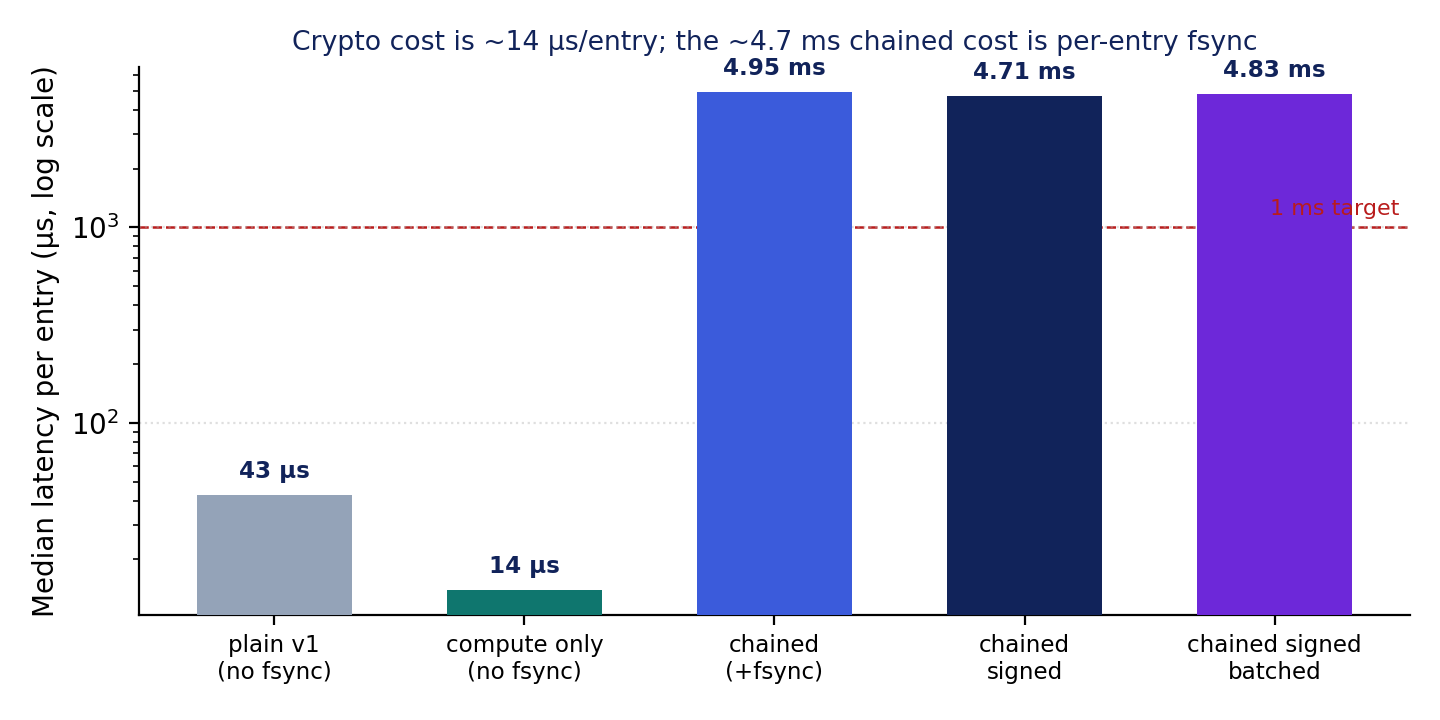
\includegraphics[width=0.95\linewidth]{figs/write_cost.png}
\caption{\textbf{Per-entry write cost by mode (log scale).} Cryptography
(\texttt{compute\_only}, \ComputeUs~\textmu s) is negligible; the
$\sim$\ChainedSignedMs~ms chained cost is the per-entry \texttt{fsync} that
guarantees fail-closed durability. Signing adds no measurable cost over chaining.
The 1~ms target is reachable on NVMe-class storage (text).}
\label{fig:write}
\end{figure}

\subsection{Anchor cadence (E3)}\label{sec:anchor}
The anchor cadence $k$ trades rollback-detection latency against external-storage
cost (Figure~\ref{fig:anchor}). Over a \AnchorN{}-entry log, every cadence detects
the rollback, and the detection window stays at or below $k$ (the RAW metric):
frequent anchoring ($k{=}10$) gives a 9-entry window at \OverheadKten{} storage,
while sparse anchoring ($k{=}10{,}000$) costs only \OverheadKtenk{} but tolerates a
$\sim$4000-entry window. \textbf{$k{=}1000$ is the sweet spot}: a
\WindowKthou{}-entry window at \OverheadKthou{} storage overhead --- comfortably
under a 1\% budget, confirming the storage hypothesis.

\begin{figure}[htb]
\centering
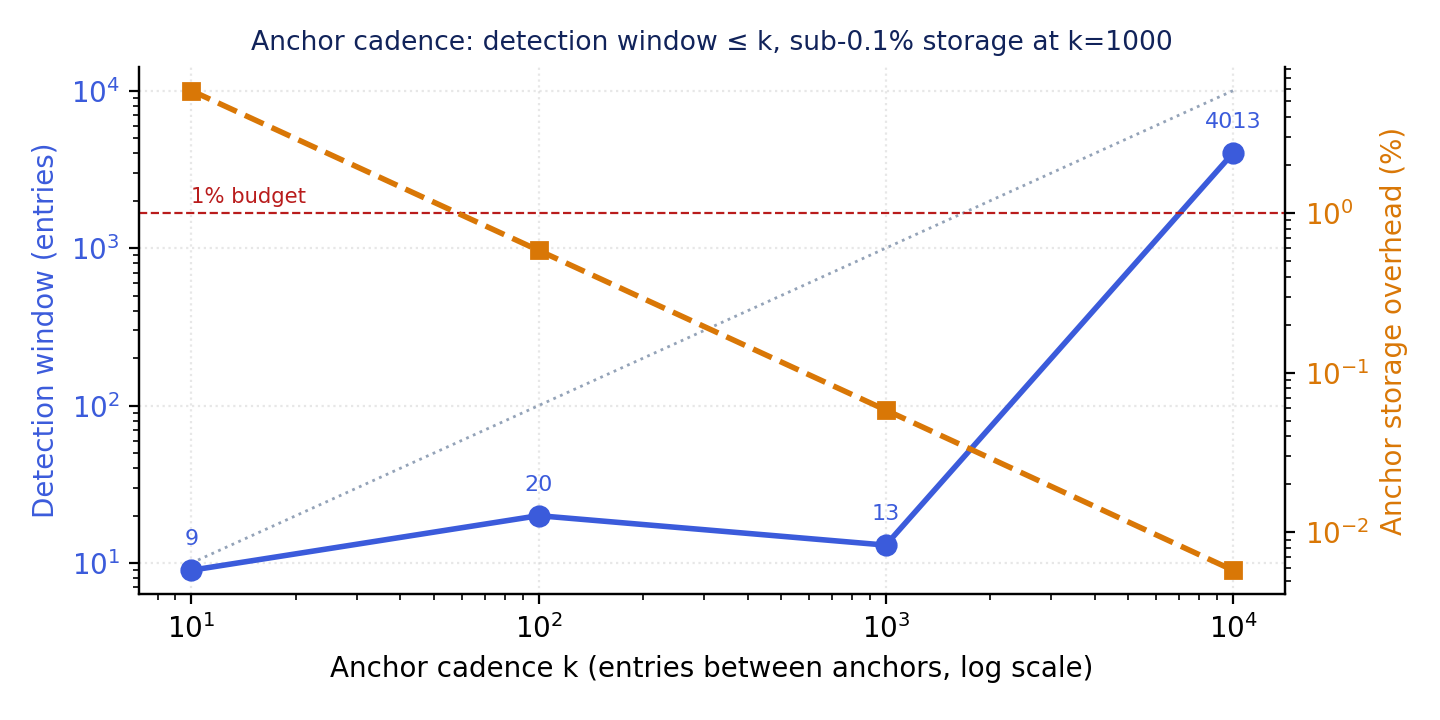
\includegraphics[width=0.95\linewidth]{figs/anchor_sweep.png}
\caption{\textbf{Anchor cadence sweep.} Detection window (left, indigo) stays under
the $k$ bound at every cadence; storage overhead (right, amber) falls below the 1\%
budget by $k{=}100$ and reaches \OverheadKthou{} at $k{=}1000$.}
\label{fig:anchor}
\end{figure}

\subsection{Verification scaling (E4)}\label{sec:verify}
Verification is linear in log size (Figure~\ref{fig:verify}) with no quadratic blowup --- the
incremental Merkle accumulator keeps anchor checking $O(n\log n)$. The unsigned chain (integrity only)
verifies at a flat $\sim$\VerifyThru~entries/s across three decades; its constant factor is a JSON parse
plus a blake3 hash per line. The security-relevant \emph{per-entry-signed} mode, verified through the
parallel+batch default (\S\ref{sec:fastverify}), sustains $\sim$\VerifyThruSigned~entries/s---\emph{within
$\sim$2$\times$ of the unsigned baseline}, rather than the $\sim$6--7$\times$ gap a sequential signature
verifier would impose. Both series are flat from $10^3$ to $10^6$.

\begin{figure}[htb]
\centering
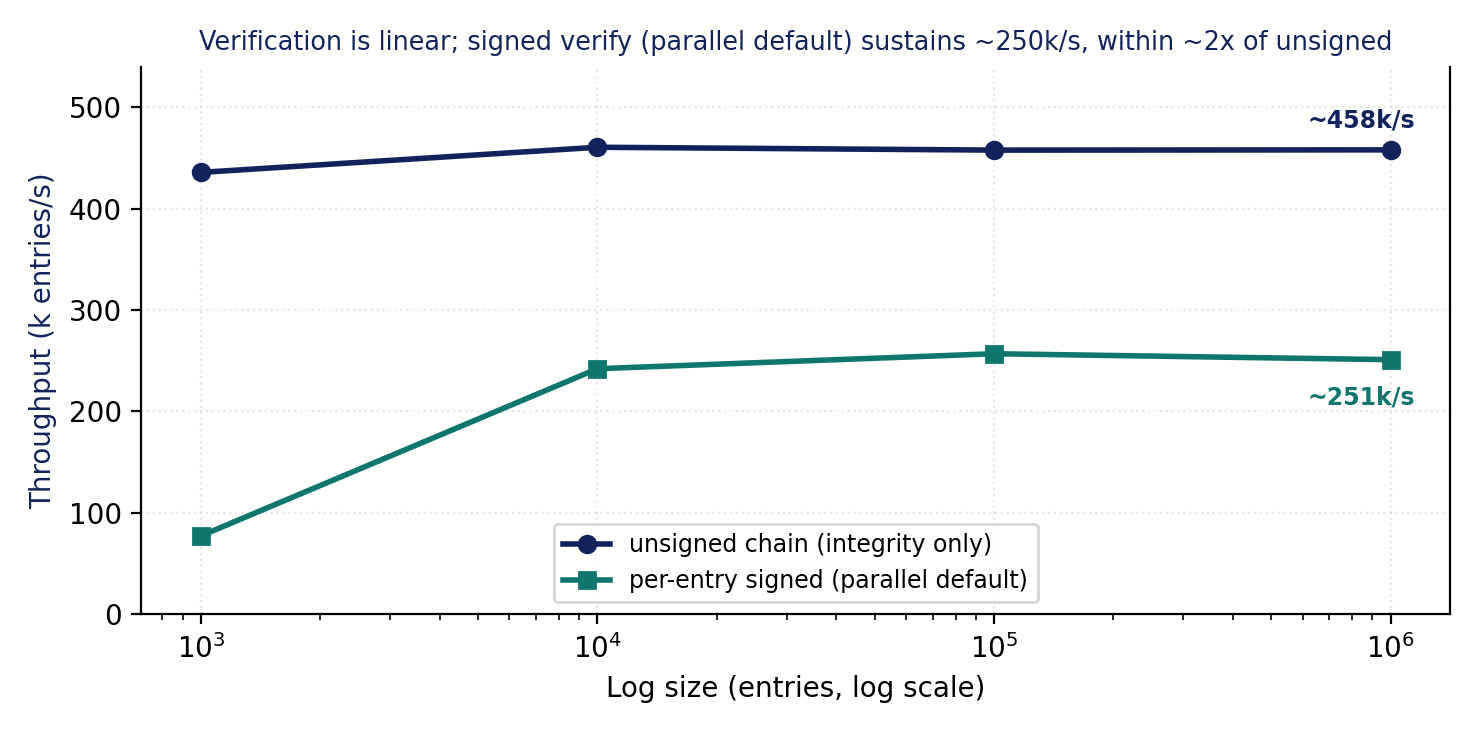
\includegraphics[width=0.95\linewidth]{figs/verify_scaling.png}
\caption{\textbf{Verification throughput vs.\ log size.} Linear (flat throughput) across three decades
for both the unsigned chain ($\sim$\VerifyThru/s) and per-entry-signed verification via the parallel+batch
default ($\sim$\VerifyThruSigned/s, \S\ref{sec:fastverify})---the latter within $\sim$2$\times$ of the former.}
\label{fig:verify}
\end{figure}

\subsection{Head-to-head with other constructions (E6)}\label{sec:compare}
We benchmark our construction against the design space of tamper-evident logging, each implemented with
\emph{identical primitives} (blake3/sha2/ed25519/hmac) on the same hardware, plus two real third-party
libraries: \texttt{ct-merkle} (an RFC~6962 Certificate Transparency append-only log~\cite{rfc6962}) and
\texttt{rs\_merkle} (a general Merkle tree). The comparison is compute-only (no fsync), isolating the
cryptographic construction from the durability tax measured in \S\ref{sec:writecost}. Figure~\ref{fig:compare}
and Table~\ref{tab:compare} report append/verify throughput, per-entry storage, third-party inclusion-proof
size, and the security properties each construction provides.

\begin{figure}[htb]\centering
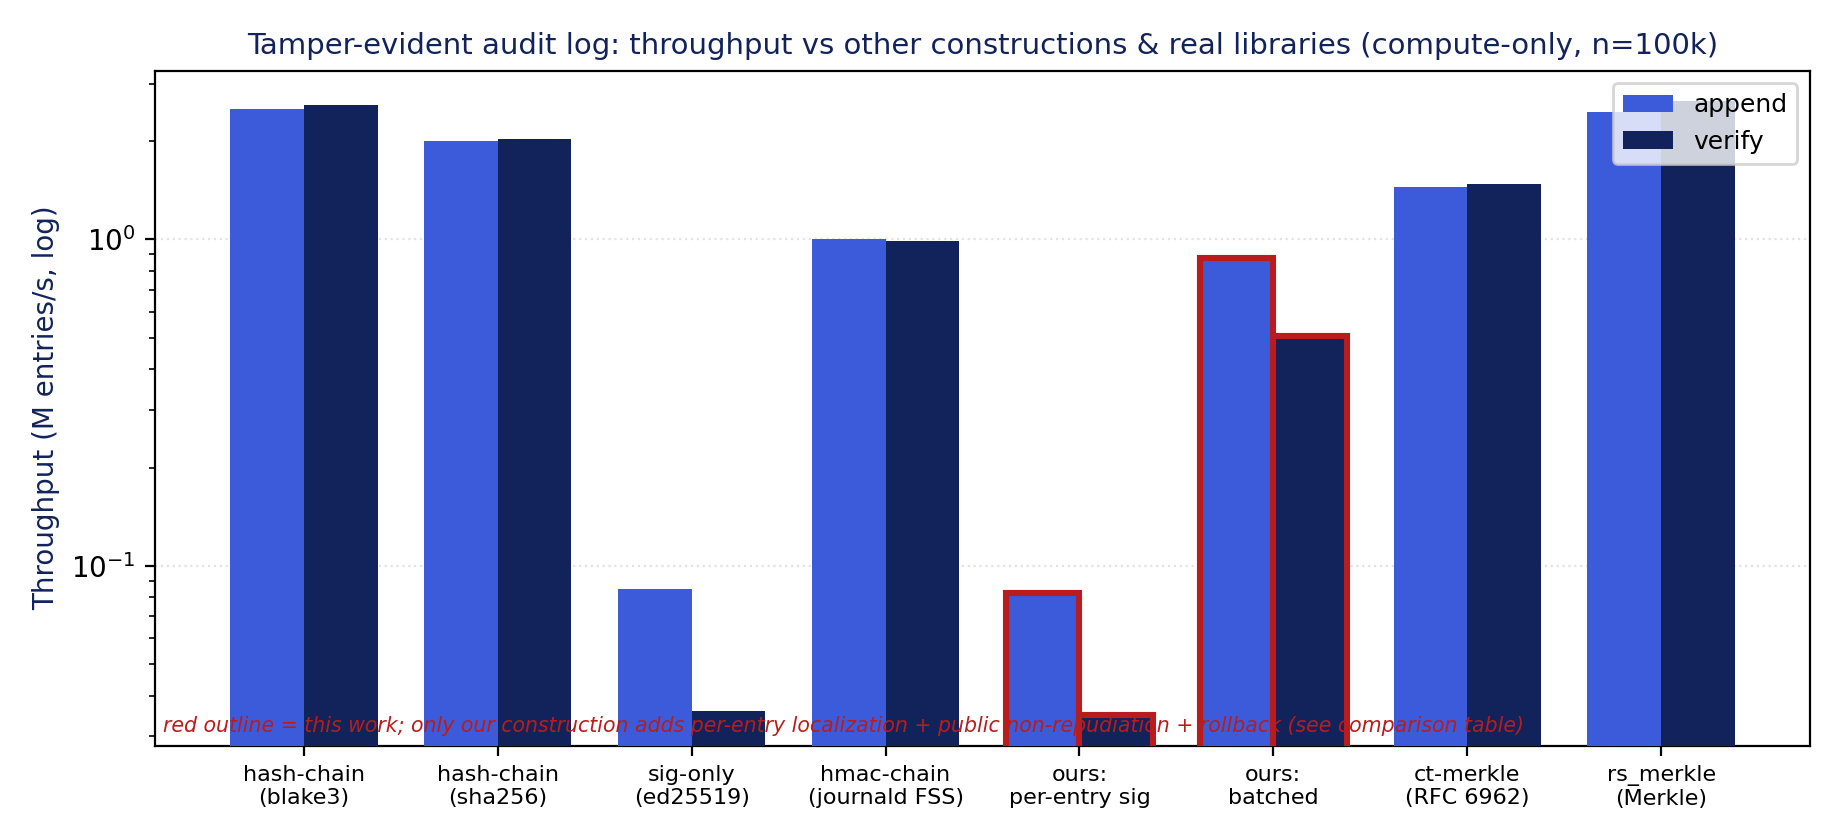
\includegraphics[width=0.98\linewidth]{figs/crypto_compare.png}
\caption{\textbf{Throughput vs.\ other constructions and real libraries} (compute-only, $n{=}100$k, best of 3).
Hash/Merkle constructions are fast; per-entry signing (ours and signature-only) is ed25519-bound. Our
\emph{batched} mode recovers most of that throughput while keeping the chain.}
\label{fig:compare}
\end{figure}

\begin{table}[htb]\centering\small
\begin{tabular}{lrrrlll}
\toprule
construction & append & verify & B/ & inclusion & public & local- \\
 & (M/s) & (M/s) & entry & proof & verif. & izes \\
\midrule
hash-chain (blake3) & 2.50 & 2.55 & 32 & $O(n)$ & integ.\ only & yes \\
hash-chain (sha256) & 1.99 & 2.01 & 32 & $O(n)$ & integ.\ only & yes \\
signature-only (ed25519) & 0.08 & 0.04 & 64 & 64\,B & yes & yes \\
hmac-chain (journald FSS) & 1.04 & 1.04 & 32 & secret & no & yes \\
\texttt{ct-merkle} (RFC 6962) & 1.46 & 1.49 & 32 & 544\,B & yes & no \\
\texttt{rs\_merkle} (Merkle) & 2.67 & 2.66 & 32 & 544\,B & yes & no \\
\textbf{ours: per-entry sig} & 0.08 & 0.04 & 96 & 96\,B & yes & yes \\
\textbf{ours: batched} & 0.89 & 0.51 & 33 & $\sim$32\,B & yes & yes \\
\bottomrule
\end{tabular}
\caption{Head-to-head (compute-only, $n{=}100$k). Inclusion proof = bytes to prove one entry to a
third-party auditor; ``localizes'' = points to the specific tampered entry (not just a batch). Only our
construction combines per-entry localization, public non-repudiation, \emph{and} rollback detection
(via the external anchor, \S\ref{sec:anchor}); the Merkle logs give compact $O(\log n)$ proofs but
localize only to a batch root, hash chains lack authenticity, and the HMAC chain is not publicly verifiable.}
\label{tab:compare}
\end{table}

\paragraph{Reading the comparison.} No construction dominates; each occupies a point in a throughput /
proof-size / security-property trade-off. Plain hash chains and Merkle logs are 3--60$\times$ faster but
provide strictly weaker guarantees for clinical audit: hash chains give integrity without authenticity,
Merkle logs localize tampering only to a batch root (not the specific action) and \texttt{rs\_merkle}
offers no rollback defense, and the HMAC chain cannot give a third-party auditor non-repudiation. Our
per-entry-signed mode is the strong, slow extreme (every action independently and publicly attributable);
our \emph{batched} mode keeps per-entry localization and the hash chain while signing Merkle checkpoints,
recovering throughput to within $\sim$3$\times$ of the Merkle libraries ($\sim$0.5\,M entries/s verify,
in the same range as the \VerifyThru/s end-to-end rate of \S\ref{sec:verify}). For a clinical record that must answer
\emph{which} action was altered and \emph{who} signed it, that property bundle---not raw throughput---is
the requirement.

\subsection{Faster verification without weakening guarantees (E7)}\label{sec:fastverify}
Per-entry signing is the verifier's \emph{only} bottleneck---blake3 chaining alone runs at $>2$\,M
entries/s (Table~\ref{tab:compare}). Crucially, ed25519 verification is per-entry-independent, so it
parallelizes and batches with \emph{zero} change to the construction: same signatures, same keys, and the
hash chain still localizes the tampered entry. The verifier therefore pre-computes signature validity off
the sequential critical path---chunked \texttt{verify\_batch} across \texttt{rayon} workers, with a
per-signature fallback inside any chunk a batch rejects, so a single bad signature is still localized to
its entry. On a 12-core machine:

\begin{table}[htb]\centering\small
\begin{tabular}{lrr}
\toprule
verification method & M sig/s & speedup\\
\midrule
sequential (per-entry) & 0.04 & 1.0$\times$\\
\texttt{rayon} parallel & 0.29 & 8.3$\times$\\
ed25519 batch & 0.11 & 3.2$\times$\\
\textbf{parallel + batch (default)} & \textbf{0.82} & \textbf{23$\times$}\\
\bottomrule
\end{tabular}
\caption{Signature-verification speedup ($n{=}100$k, 12 cores, best of 3). The verifier now defaults to
parallel+batch, taking per-entry-signed verification from the slowest construction to faster than our own
batched mode and within $\sim$2$\times$ of the Merkle libraries (Table~\ref{tab:compare})---while keeping
per-entry public non-repudiation. Detection and localization are unchanged (E1: 26/26 detected, 20/20
localized); the result is cryptographically identical to sequential verification.}
\label{tab:fastverify}
\end{table}

This makes the strong, fully-attributable per-entry-signed mode a practical default rather than a slow
extreme: it now verifies an order of magnitude faster while still naming the specific tampered action and
the key that signed it.

% ============================================================================
\section{Security Argument}\label{sec:security}
Integrity and non-repudiation reduce to two standard assumptions. \emph{Chain
integrity}: any modification of a recorded entry changes its prefix bytes, so
detection fails only under a blake3 collision; tamper-evidence thus reduces to the
collision-resistance of blake3~\cite{blake3}. \emph{Non-repudiation}: each entry's
hash is signed with ed25519, so a verifier holding the public key cannot forge a
valid signature, and a recorded action cannot be repudiated unless the EUF-CMA
security of ed25519~\cite{ed25519} is broken --- a property a shared MAC cannot
provide, since any MAC holder could forge. Per adversary tier: tiers (i) the agent
and (ii) a co-located process cannot produce a self-consistent chain without the
signing key, so TA1--TA5 are caught immediately; tier (iii) a privileged operator
who also obtains the key can re-emit a consistent log, but cannot reproduce the
external anchors (TA6 caught within $k$) and cannot re-sign under the real key seen
by a verifier with a pinned public key (downgrade caught). Timestamps are recorded
but never trusted for ordering --- the sequence number is the order --- so
backdating (TA4) is a sequence/forgery violation, not a clock-trust question.

% ============================================================================
\section{Discussion and Limitations}\label{sec:limitations}
\paragraph{Relationship to HAARF.} This work is the primary owner of HAARF category
\textbf{C2} (end-to-end traceability and non-repudiable audit), and supports C8's
authorization-evidence requirements by making every gateway decision a signed,
ordered, externally-anchored record~\cite{schwoebel2026haarf}.

\paragraph{Honest performance framing.} Two pre-registered targets are not met on
the development machine and we report them as such rather than re-scope them.
Per-entry \texttt{fsync} makes chained writes $\sim$\ChainedSignedMs~ms (the correct
fail-closed semantic; sub-millisecond is NVMe-class, \S\ref{sec:writecost}), and a
$10^6$-entry verify takes \VerifyOneM~s on one core (linear, parallelizable,
\S\ref{sec:verify}). Both gaps are constant-factor and hardware/parallelism-bound,
not algorithmic.

\paragraph{Other limitations.} (a) Full-file rewrite with the signing key is
defended only by anchoring and a pinned verifier key, not by the chain alone. (b)
Signed external timestamps are future work; we record but do not trust wall-clock
time. (c) Key management (HSM/KMS, attestation release) follows the QUOKKAGUARD
pattern and is discussed, not benchmarked here. (d) A log with a trailing incomplete
batch has uncheckpointed tail entries; the verifier surfaces this via a
\texttt{signatures\_checked} flag rather than silently treating the tail as
verified. (e) Action streams are synthetic; realism of the modeled clinical
workflow is a threat to external validity, addressed by the schema review in the
proposal.

% ============================================================================
\section{Conclusion}
The record of what a clinical AI agent did is the foundation of every governance
claim made about it, and until now this program left that record mutable. We made it
tamper-evident: a unified, blake3-chained, ed25519-signed, externally-anchored,
fail-closed log with a localizing verifier, detecting \TDR{} of tampering at a
cryptographic cost of \ComputeUs~\textmu s/entry. Non-repudiable provenance is not
the expensive part of trustworthy clinical AI --- durability is --- and durability
is a deployment choice, not a research obstacle. The next layer in the program
builds context-aware authorization (quwarden) on top of this evidence base.

% ============================================================================
\section*{Declaration of generative AI use}
During the preparation of this work the author used \emph{Claude (Anthropic)} as a
coding and drafting assistant --- for implementing and reviewing the Rust audit
module under test-driven development, generating the figure-plotting and
experiment-driver code, and drafting and copy-editing this manuscript. After using
this tool, the author reviewed and edited all content and takes full responsibility
for the publication. No generative-AI system was used to generate or fabricate
experimental data, interpret results, or produce clinical conclusions, and no AI
tool is listed as an author, as such tools do not satisfy authorship criteria.

\section*{Data and code availability}
All code, the TamperBench generator and corpus, and result artifacts are available
at \href{https://github.com/quome-cloud/quledger}{\nolinkurl{github.com/quome-cloud/quledger}}
under the Apache-2.0 license. All patient data are synthetic; no real protected
health information was used.

\section*{Author contributions}
J.S.\ conceived the study, designed and implemented the system, ran the experiments,
and wrote the manuscript.

\section*{Competing interests}
The author is affiliated with Quome Inc. The author declares no other competing
interests.

\section*{Funding}
This work received no specific external funding.

% ============================================================================
\appendix
\section{Detailed result tables}\label{app:tables}
\begin{table}[htb]\centering\small
\begin{tabular}{lrrl}
\toprule
Write mode & Median/entry & vs.\ plain & What it includes \\
\midrule
plain v1 (no fsync) & \PlainUs~\textmu s & 1.0$\times$ & JSONL append, no durability \\
compute only (no fsync) & \ComputeUs~\textmu s & 0.3$\times$ & blake3 + ed25519, no I/O \\
chained (+fsync) & \ChainedMs~ms & $\sim$116$\times$ & + per-entry fsync \\
chained signed & \ChainedSignedMs~ms & $\sim$110$\times$ & + ed25519 per entry + fsync \\
chained signed batched & 4.83~ms & $\sim$113$\times$ & + batched checkpoint sigs + fsync \\
\bottomrule
\end{tabular}
\caption{E2 write cost per mode (medians, dev HW). The two-order-of-magnitude jump
is per-entry \texttt{fsync}, not cryptography.}
\label{tab:write}
\end{table}

\begin{table}[htb]\centering\small
\begin{tabular}{rrrrl}
\toprule
$k$ & anchors & detection window & storage overhead & detected \\
\midrule
10 & 2000 & 9 & \OverheadKten{} & yes \\
100 & 200 & 20 & \OverheadKhund{} & yes \\
1000 & 20 & \WindowKthou{} & \OverheadKthou{} & yes \\
10000 & 2 & 4013 & 0.006\% & yes \\
\bottomrule
\end{tabular}
\caption{E3 anchor cadence sweep over a \AnchorN{}-entry log. Window $\le k$ at every
cadence; storage under 1\% from $k{=}100$.}
\label{tab:anchor}
\end{table}

\section{Reproducibility}\label{app:reproduce}
A single environment (Rust 2021 + Python 3 stdlib + \texttt{matplotlib}; no API
keys) reproduces every result.
\begin{lstlisting}[style=housespecyamlbare]
cargo build --release
python3 scripts/003-tamper-audit/e1_detection.py        # E1/E5 -> summary.json
cargo bench --bench audit_write                          # E2
cargo bench --bench audit_verify                         # E4
python3 scripts/003-tamper-audit/e3_anchor_sweep.py \
    > results/003-tamper-audit/e3_anchor/e3_anchor_sweep.csv   # E3
python3 scripts/003-tamper-audit/make_figs.py            # figures
cd papers/003-tamper-audit && make paper                 # this PDF
\end{lstlisting}
All randomized steps use seed 42; result artifacts are written under
\texttt{results/003-tamper-audit/}.

\clearpage
\bibliographystyle{plain}
\bibliography{refs}
\end{document}
